% Copyright (c) 2017 Ongun Kanat <ongun.kanat@gmail.com>
% Permission is hereby granted, free of charge, to any person obtaining a copy of 
% this software and associated documentation files (the "Software"), to deal in 
% the Software without restriction, including without limitation the rights to 
% use, copy, modify, merge, publish, distribute, sublicense, and/or sell copies of 
% the Software, and to permit persons to whom the Software is furnished to do so, 
% subject to the following conditions:
% 
% The above copyright notice and this permission notice shall be included in all 
% copies or substantial portions of the Software.
% 
% THE SOFTWARE IS PROVIDED "AS IS", WITHOUT WARRANTY OF ANY KIND, EXPRESS OR 
% IMPLIED, INCLUDING BUT NOT LIMITED TO THE WARRANTIES OF MERCHANTABILITY, FITNESS 
% FOR A PARTICULAR PURPOSE AND NONINFRINGEMENT. IN NO EVENT SHALL THE AUTHORS OR 
% COPYRIGHT HOLDERS BE LIABLE FOR ANY CLAIM, DAMAGES OR OTHER LIABILITY, WHETHER 
% IN AN ACTION OF CONTRACT, TORT OR OTHERWISE, ARISING FROM, OUT OF OR IN 
% CONNECTION WITH THE SOFTWARE OR THE USE OR OTHER DEALINGS IN THE SOFTWARE.

% 12pt and ISO A4 paper with title page add notitlepage for otherwise
\documentclass[a4paper, 12pt, titlepage]{article}

% Margins and page size
\usepackage[a4paper,top=2.5cm,bottom=2.5cm,left=3.3cm,right=2.2cm]{geometry}

% Page headers are set to top right
\usepackage{fancyhdr}
\pagestyle{fancy}
\setlength{\headheight}{15pt}
\renewcommand{\footrulewidth}{0pt} % clear rulers
\renewcommand{\headrulewidth}{0pt}
\lhead{} % Empty left header
\rhead{\thepage} % Page number at the right header
\cfoot{} % Clear center of the footer

% Use American English for dates etc.
%\usepackage[american]{babel}
% If document is in Turkish then use
% \usepackage[turkish]{babel}
% or for both
\usepackage[turkish,american]{babel}

% Indent at section beginnings
%\usepackage{indentfirst}

% utf-8 support
\usepackage[utf8]{inputenc}


% Figure placement
\usepackage{float}

% An enumeration package for flexible enumeration
\usepackage{enumitem}

% Helvetica Sans-serif fonts
\usepackage{helvet}
\usepackage{sectsty}
\allsectionsfont{\normalfont\sffamily\bfseries}
\sectionfont{\fontsize{18pt}{21.6pt}\sffamily\bfseries}
\subsectionfont{\fontsize{16pt}{19.2pt}\sffamily\bfseries}
\subsubsectionfont{\fontsize{14pt}{16.8pt}\sffamily\bfseries}

% Paragraph spacings
\setlength{\parindent}{0pt}
\setlength{\parskip}{12pt}

% Courier monospace font
\usepackage{courier}

% Table of contents dot fill
\usepackage{tocloft}
\renewcommand{\cftsecleader}{\cftdotfill{\cftdotsep}}
\tocloftpagestyle{fancy}
\renewcommand{\cfttoctitlefont}{\sffamily\Large\bfseries}
\setlength{\cftbeforesecskip}{6pt}

% Links, both local and external
\usepackage{hyperref}
\hypersetup{
    unicode=true,
    colorlinks=true,
    urlcolor=blue,
    citecolor=black,
    menucolor=black,
    linkcolor=black
}

% Figure captions are bold
\usepackage[labelfont=bf,font=sf]{caption}


% Pseudocode from algorithmicx package
\usepackage{algorithmicx}
\usepackage{algpseudocode}
\usepackage[section,boxed]{algorithm}
\captionsetup[algorithm]{labelfont=bf,font=sf,justification=centering,position=top}

% For fitting tables into the page width
\usepackage{makecell}
\renewcommand{\theadalign}{cc} % Centering and at the middle
\renewcommand{\theadfont}{\bfseries} % Bold table headers
\usepackage{tabularx}
\newcolumntype{Y}{>{\centering\arraybackslash}X}

% Listings for implemented code
\usepackage{listings}
\lstset{basicstyle=\ttfamily,frame=lines,tabsize=4}
\renewcommand{\lstlistingname}{Listing}
\lstset{
    breakatwhitespace=false,
    breaklines=true,
    captionpos=b,
    escapeinside={\%*}{*)},
    frame=single,
    keepspaces=true,
    numbers=left,
    numbersep=5pt,
    xleftmargin=8pt,
}

% A powerful math notation package
\usepackage{amsmath}

% Override here with the names
\newcommand{\thetitle}{TinyNPU}
\newcommand{\theturkishtitle}{TinyNPU}
\newcommand{\theauthor}{Fırat Kızılboğa}
\newcommand{\thestudentid}{150200115}
\newcommand{\thedate}{March 2026}
\newcommand{\theturkishdate}{Mart 2026}
\newcommand{\theadvisor}{Assoc. Prof. Dr. Ayse Yilmazer}

\usepackage{color}
\definecolor{darkgreen}{RGB}{0, 128, ,0}
\newcommand{\fixme}[1]{{\color{red}\bfseries\sffamily (FIXME: #1)}}
\newcommand{\suggest}[1]{{\color{darkgreen}\bfseries\sffamily (SUGGESTION: #1)}}
\newcommand{\ask}[1]{{\color{blue}\bfseries\sffamily (QUESTION: #1)}}

\newcommand\Includegraphics{\expandafter\includegraphics\expandafter} 

% Title, author and date info
\title{\thetitle}
\author{\theauthor}
\date{\thedate}

% Graphics for PDFTeX
\usepackage{graphicx}


\begin{document}
\numberwithin{figure}{section}
\numberwithin{table}{section}
\numberwithin{lstlisting}{section}
\shorthandoff{=}


\begin{titlepage}
    \bfseries % Make all text bold in this environment
    \sffamily % Similarly select sans-serif font
    \begin{center}
        \LARGE{\textbf{ISTANBUL TECHNICAL UNIVERSITY \\ 
               FACULTY OF COMPUTER AND INFORMATICS} } \\
        \vspace{5.5cm}
        \LARGE{\thetitle}  \\
        \vspace{4.5cm}
        \Large{Graduation Project Final Report} \\
        \vspace{0.5cm}
        \Large{\theauthor} \\
        \Large{\thestudentid} \\
        \vspace{4cm}
        \large{Department: Computer Engineering} \\
        \large{Division: Computer Engineering} \\
        \vspace{1.5cm}
        \large{Advisor: \theadvisor} \\
        \vspace{\fill} % Fill out until the page end
        \large{\normalfont \sffamily \thedate}
    \end{center}
\end{titlepage}

\pagenumbering{Roman} % Capital roman numerals as page numbers
\newpage
\section*{Statement of Authenticity}
I/we hereby declare that in this study
\begin{enumerate}
    \item all the content influenced from external references are cited clearly and in detail,
    \item and all the remaining sections, especially the theoretical studies and implemented software/hardware that constitute the fundamental essence of this study is originated by my/our individual authenticity.
\end{enumerate}
\vspace{1em}
İstanbul, \theturkishdate
\vspace{3em}\\ \theauthor

\newpage
\section*{Acknowledgments}
I would like to thank my advisor, Assoc. Prof. Dr. Ayse Yilmazer, for her guidance throughout this project. I also thank the people whose open-source tooling and research made it possible to build, analyze, and validate the TinyNPU hardware and software stack.

\newpage
\section*{\centering\thetitle}
\centerline{\fontsize{16pt}{21.6pt}\sffamily\bfseries (SUMMARY)}
TinyNPU is a compact accelerator project that evolved into a complete hardware/software stack. The project now includes a parameterized systolic-array-based neural processing unit, a PyTorch-first segmented compiler and runtime, a quantization-aware model preparation flow, RTL and host-side verification infrastructure, and performance and synthesis characterization tooling. The goal of the project is not merely to design a datapath, but to make that datapath usable from a realistic machine-learning workflow and measurable in a disciplined way.

The hardware architecture is organized around an $N \times N$ output-stationary systolic array, a unified buffer, an instruction memory, streamer logic that feeds the array, and a post-processing unit that applies bias, rescaling, activation, and packed writeback. The software stack traces PyTorch models, partitions them into accelerator segments and host operations, compiles supported segments into TinyNPU instruction and buffer images, and executes the resulting plan on either host emulation or RTL simulation. Unsupported work is never hidden; it appears explicitly as host-side steps in the execution plan.

One of the main lessons of the project is that the useful unit of design is the whole stack, not the RTL alone. Compiler-visible tensor semantics, physical packing format, host/NPU boundaries, verification points, and repeated-run runtime behavior all affect whether the accelerator is practical to use. For this reason, the project includes explicit host-op dispatch, compiler-owned expected tensors for verification, repeated-run sessions with persistent state, and benchmark accounting that separates accelerator compute cycles from runtime and protocol overhead.

The current experimental evidence is intentionally narrow but concrete. The implemented stack has been validated end-to-end on a trained MNIST model, and a controlled multi-tile matrix multiplication benchmark has been used to study compute speedup and integration overhead. In addition, a reproducible Yosys-based synthesis flow provides rough resource estimates for the current design. The report therefore presents TinyNPU not as a finished industrial inference platform, but as a working accelerator research system whose main value lies in understanding architecture, compilation, packing, and workload fit together.

\newpage
\section*{\centering\theturkishtitle}
\centerline{\fontsize{16pt}{21.6pt}\sffamily\bfseries (ÖZET)}
TinyNPU, özel bir nöral işlemci birimi ile onu kullanılabilir hale getiren derleyici, çalışma zamanı, niceleme akışı ve benzetim tabanlı doğrulama ortamını birlikte geliştirmeyi amaçlayan bir projedir. Projenin hedefi yalnızca küçük bir hızlandırıcı çekirdeği tasarlamak değil, bu çekirdeği gerçek bir makine öğrenmesi iş akışında kullanılabilir hale getirmektir. Bu nedenle proje, PyTorch tabanlı model hazırlama sürecini destekleyen, nicelemeli modelleri hızlandırıcı segmentlerine dönüştüren, desteklenmeyen işlemleri ana işlemci üzerinde çalıştıran ve sonuçları yazılım referanslarıyla doğrulayan bütünleşik bir donanım-yazılım yapısı içermektedir.

Donanım tarafında TinyNPU, birleşik tampon bellek ve komut belleği ile beslenen sistolik dizi tabanlı bir hesaplama çekirdeği etrafında kurulmuştur. Girdi aktivasyonları ve ağırlıklar birleşik tampondan akıtıcı birimlere, oradan da sistolik diziye iletilir. Hesaplama sonucunda oluşan değerler son işleme biriminden geçirilerek paketlenmiş biçimde tekrar belleğe yazılır. Bu yapı, yoğun nicelemeli matris işlemleri için verimli bir veri yolu sağlarken, dışarıdan görülen programlama modelini de yönetilebilir düzeyde tutmaktadır. Yazılım tarafı ise yüksek seviyeli model işlemlerini hızlandırıcı segmentleri ve gerekirse ana işlemci işlemlerini birlikte içeren bir yürütme planına dönüştürmektedir.

Bu projedeki temel ilerleme, izole donanım deneylerinden uçtan uca çalışan bir sisteme geçilmesi olmuştur. Eğitilmiş MNIST modeli dahil gerçek iş yükleri yazılım ve donanım yığını üzerinden çalıştırılabilmektedir. Ayrıca, hızlandırıcının gerçek hesaplama çevrimlerini entegrasyon ek yüklerinden ayıran bir ölçüm altyapısı geliştirilmiştir. Böylece çekirdeğin kendi verimliliği ile yazılım, paketleme ve arayüz maliyetleri ayrı ayrı değerlendirilebilmektedir. Tekrarlı çıkarım senaryolarında gereksiz durum yüklemelerini azaltmak için oturum tabanlı çalışma ve ağırlık kalıcılığı desteği de eklenmiştir.

Projenin mevcut durumu, donanımın anlamlı hesaplama yaptığı, ancak sistem seviyesindeki davranışın derleyici bölütlemesi, bellek yerleşimi ve çalışma zamanı düzenlemesine güçlü biçimde bağlı olduğunu göstermektedir. Bu nedenle proje, ``derleyiciyi var etmek'' aşamasını aşmış; bunun yerine derleyici ve çalışma zamanının karmaşıklığını yönetmek, gereksiz çevrim maliyetlerini azaltmak ve hangi iş yüklerinin bu mimariye uygun olduğunu anlamak gibi daha olgun tasarım sorularına yönelmiştir. Bu rapor, ortaya çıkan sistemi, temel tasarım kararlarını ve işlevsellik ile performans değerlendirmesinde kullanılan yöntemi özetlemektedir.

\newpage
\tableofcontents
\newpage

% For the ones who doesn't know: 1,2,..9 called West Arabic numbers
\pagenumbering{arabic}
\section{Introduction and Project Summary}
\subsection{Background and Motivation}
Modern deep neural networks demand substantial compute and memory bandwidth even at inference time. This has made specialized accelerator design a central topic both for datacenter-scale systems and for smaller edge-oriented deployments \cite{jouppi2017datacenter, genc2021gemmini}. Quantization is one of the main techniques that makes such deployment practical, because it reduces memory traffic and allows arithmetic throughput to increase when narrow integer types are used instead of floating-point data.

However, quantization is not a single fixed target. Mixed-precision work has shown that different layers or kernels inside the same model can tolerate different bit-widths \cite{wu2018mixedprecision}. This creates a hardware opportunity and a software problem at the same time. Hardware should benefit from narrower arithmetic when it is safe to do so, but the software stack must still prepare the model, preserve numerical intent, and decide where accelerator execution ends and host execution begins.

\subsection{Problem Definition}
The main problem addressed by TinyNPU is therefore not only how to build a small systolic-array accelerator, but how to make mixed-precision quantized computation usable from a realistic model flow. Fixed-precision accelerators leave throughput on the table when different parts of a model have different precision needs. At the other end of the spectrum, CPU-centric approaches based on ISA extensions or soft SIMD can support low-bit computation, but they still pay substantial software-side cost for packing, unpacking, and orchestrating the data movement around those operations \cite{garofalo2021xpulpnn, armeniakos2024mixedprecision, fornt2025mixgemm}.

This project treats the problem as a co-design task. The hardware must expose a regular datapath that benefits from packed low-precision arithmetic. The compiler and runtime must make tensor layout, quantization boundaries, and host fallbacks explicit rather than implicit. The result should be a system that can be measured honestly: accelerator compute, runtime overhead, and host-side work should not be conflated.

\subsection{Project Scope and Approach}
TinyNPU approaches this problem with four coupled components:
\begin{enumerate}
    \item \textbf{A parameterized mixed-precision accelerator:} TinyNPU is centered around an output-stationary $N \times N$ systolic array, a unified buffer, streamer logic that feeds the array, and a post-processing unit that performs bias addition, rescaling, activation, saturation, and packed writeback.
    \item \textbf{Packed integer computation:} The processing elements support packed INT16, INT8, and INT4 execution modes. Throughput therefore scales with precision reduction, not by changing the global architecture, but by packing more useful work into the same datapath.
    \item \textbf{A segmented compiler/runtime:} The software flow traces supported PyTorch models, partitions them into accelerator segments and explicit host-side operations, lowers legal accelerator work into instruction and buffer images, and executes the resulting plan on either host emulation or RTL simulation.
    \item \textbf{Verification and measurement infrastructure:} The project includes compiler-owned expected tensors, runtime verification points, repeated-run sessions, and benchmark accounting that separates accelerator compute from protocol and software overhead.
\end{enumerate}

The current project state should be read with that scope in mind. TinyNPU is already capable of running a trained MNIST model through the full compiler/runtime stack and of benchmarking a controlled multi-tile matrix multiplication workload. At the same time, workload coverage is still narrow, and the current results are most useful for understanding architecture, packing, compiler boundaries, and runtime cost rather than for claiming broad deployment readiness.

The rest of this report follows that logic. The next section positions TinyNPU relative to relevant literature in mixed-precision quantization, matrix multiplication, and accelerator design. The system model section then explains the implemented hardware and software stack in detail, followed by the experimental method, the current results, and the most important next steps.
\newpage

\section{Comparative Literature Survey}
\subsection{Mixed-Precision Quantization}
Mixed-precision quantization work is the clearest algorithmic motivation for TinyNPU. Wu et al. formulate layer-wise quantization as a search problem and show that different layers can be assigned different bit-widths without treating the whole model uniformly \cite{wu2018mixedprecision}. This is the key observation behind a variable-precision accelerator: if model layers do not all need the same precision, a fixed-precision datapath cannot exploit the full efficiency opportunity.

Quantization is also relevant as a compiler concern rather than only a hardware concern. SmoothQuant is an example of pushing difficult numerical adjustments into an offline transformation so that runtime execution becomes simpler and more hardware-friendly \cite{xiao2023smoothquant}. TinyNPU follows the same general philosophy even though it does not implement the full SmoothQuant method itself: model preparation, fused rescaling, and compiler-ready conversion are treated as software responsibilities that simplify the accelerator contract.

\subsection{High-Performance Matrix Multiplication}
The mathematical core of TinyNPU is still matrix-style computation, so the project is strongly informed by classical GEMM literature. Goto and van de Geijn show that high-performance matrix multiplication depends not only on arithmetic throughput, but on careful tiling and data movement through the memory hierarchy \cite{goto2008anatomy}. The same principle appears in TinyNPU at a smaller scale. When matrices exceed the dimensions of the systolic array, the compiler and runtime must tile along the $M$, $N$, and $K$ dimensions while preserving the data reuse pattern expected by the array and its post-processing path.

\subsection{Existing Accelerator Architectures}
On the accelerator side, Google's TPU remains the canonical reference for systolic-array-style matrix acceleration \cite{jouppi2017datacenter}. Gemmini is especially relevant because it demonstrates how a systolic array, programming model, and system context can be treated as one full-stack research object rather than as an isolated RTL block \cite{genc2021gemmini}. That full-stack perspective is one of the strongest methodological reference points for TinyNPU.

An earlier educational TinyTPU implementation was useful as a starting point for understanding systolic-array organization, but it was not a good endpoint for this project. Extending it toward mixed precision, tiled execution, and cleaner post-processing exposed the limits of treating the datapath as the whole problem. TinyNPU therefore diverged into a custom implementation with a different software contract, explicit host/accelerator boundaries, and a compiler/runtime that owns packing and verification rather than leaving those concerns informal.

Taken together, these references define the design space in which TinyNPU sits. It is not trying to outscale large industrial accelerators. Its niche is a compact mixed-precision accelerator system in which the hardware, packing model, compiler/runtime, and measurement methodology can all be studied together in one working platform.
\newpage

\section{Developed Approach and System Model}
The developed system consists of four tightly coupled parts: the RTL accelerator, the model preparation and quantization flow, the segmented JIT compiler/runtime, and the verification and benchmarking infrastructure. These pieces were built together because no single layer is meaningful in isolation. The hardware cannot be evaluated honestly without a realistic execution path, and the compiler cannot be trusted without RTL-backed validation.
\subsection{Data Model}
The core data model is built around explicit tensors, explicit quantization metadata, and explicit execution-plan artifacts. In the segmented compiler flow, each tensor is represented by a typed specification carrying shape, data type, tensor kind, optional constant data, verification intent, and metadata such as quantization parameters. This is important because TinyNPU does not operate on generic floating-point tensors at runtime. The compiler and runtime need to know exactly when a tensor is a floating host value, when it is a signed quantized value, and when it has already been converted into a packed accelerator-facing representation.

The next major data structure is the execution plan. Rather than generating a monolithic ``program'' for the whole model, the compiler builds an \texttt{ExecutionPlan} whose steps are typed as \texttt{NpuSegment}, \texttt{HostOp}, or \texttt{VerifyTensor}. \texttt{NpuSegment} groups together accelerator-supported matrix-style work. \texttt{HostOp} keeps unsupported or intentionally host-side work explicit. \texttt{VerifyTensor} allows compiler-owned expected tensors to be checked at runtime. This split is central to the project because it makes boundaries and fallback semantics visible instead of implicit.

Physical layout is also part of the data model. The current backend uses role-specific packings for tensors that feed the array horizontally, tensors that feed it vertically, output buffers that match the writeback layout, and packed bias vectors. These layouts are backend details rather than semantic tensor meanings, but they matter because the compiler must map logical tensors onto physical storage forms that match the datapath. A large part of the compiler work came from keeping this physical reality explicit without allowing it to leak upward and distort the logical semantics of the graph.
\subsection{Structural Model}
Structurally, TinyNPU is organized around a control path and a compute path. The control path is responsible for instruction orchestration and host service. In the current runtime path, data staging is primarily handled through the shared-SRAM host window, while MMIO commands remain the control path for launch/status and compatibility fallback. The compute path consists of the unified buffer, streamer logic, a parameterized $N \times N$ output-stationary systolic array, and the post-processing unit. During active computation, data is read from the unified buffer, transformed into the orientation expected by the array, consumed by the processing elements, and then drained through the post-processing unit before being written back in packed form.

\begin{figure}[H]
    \centering
    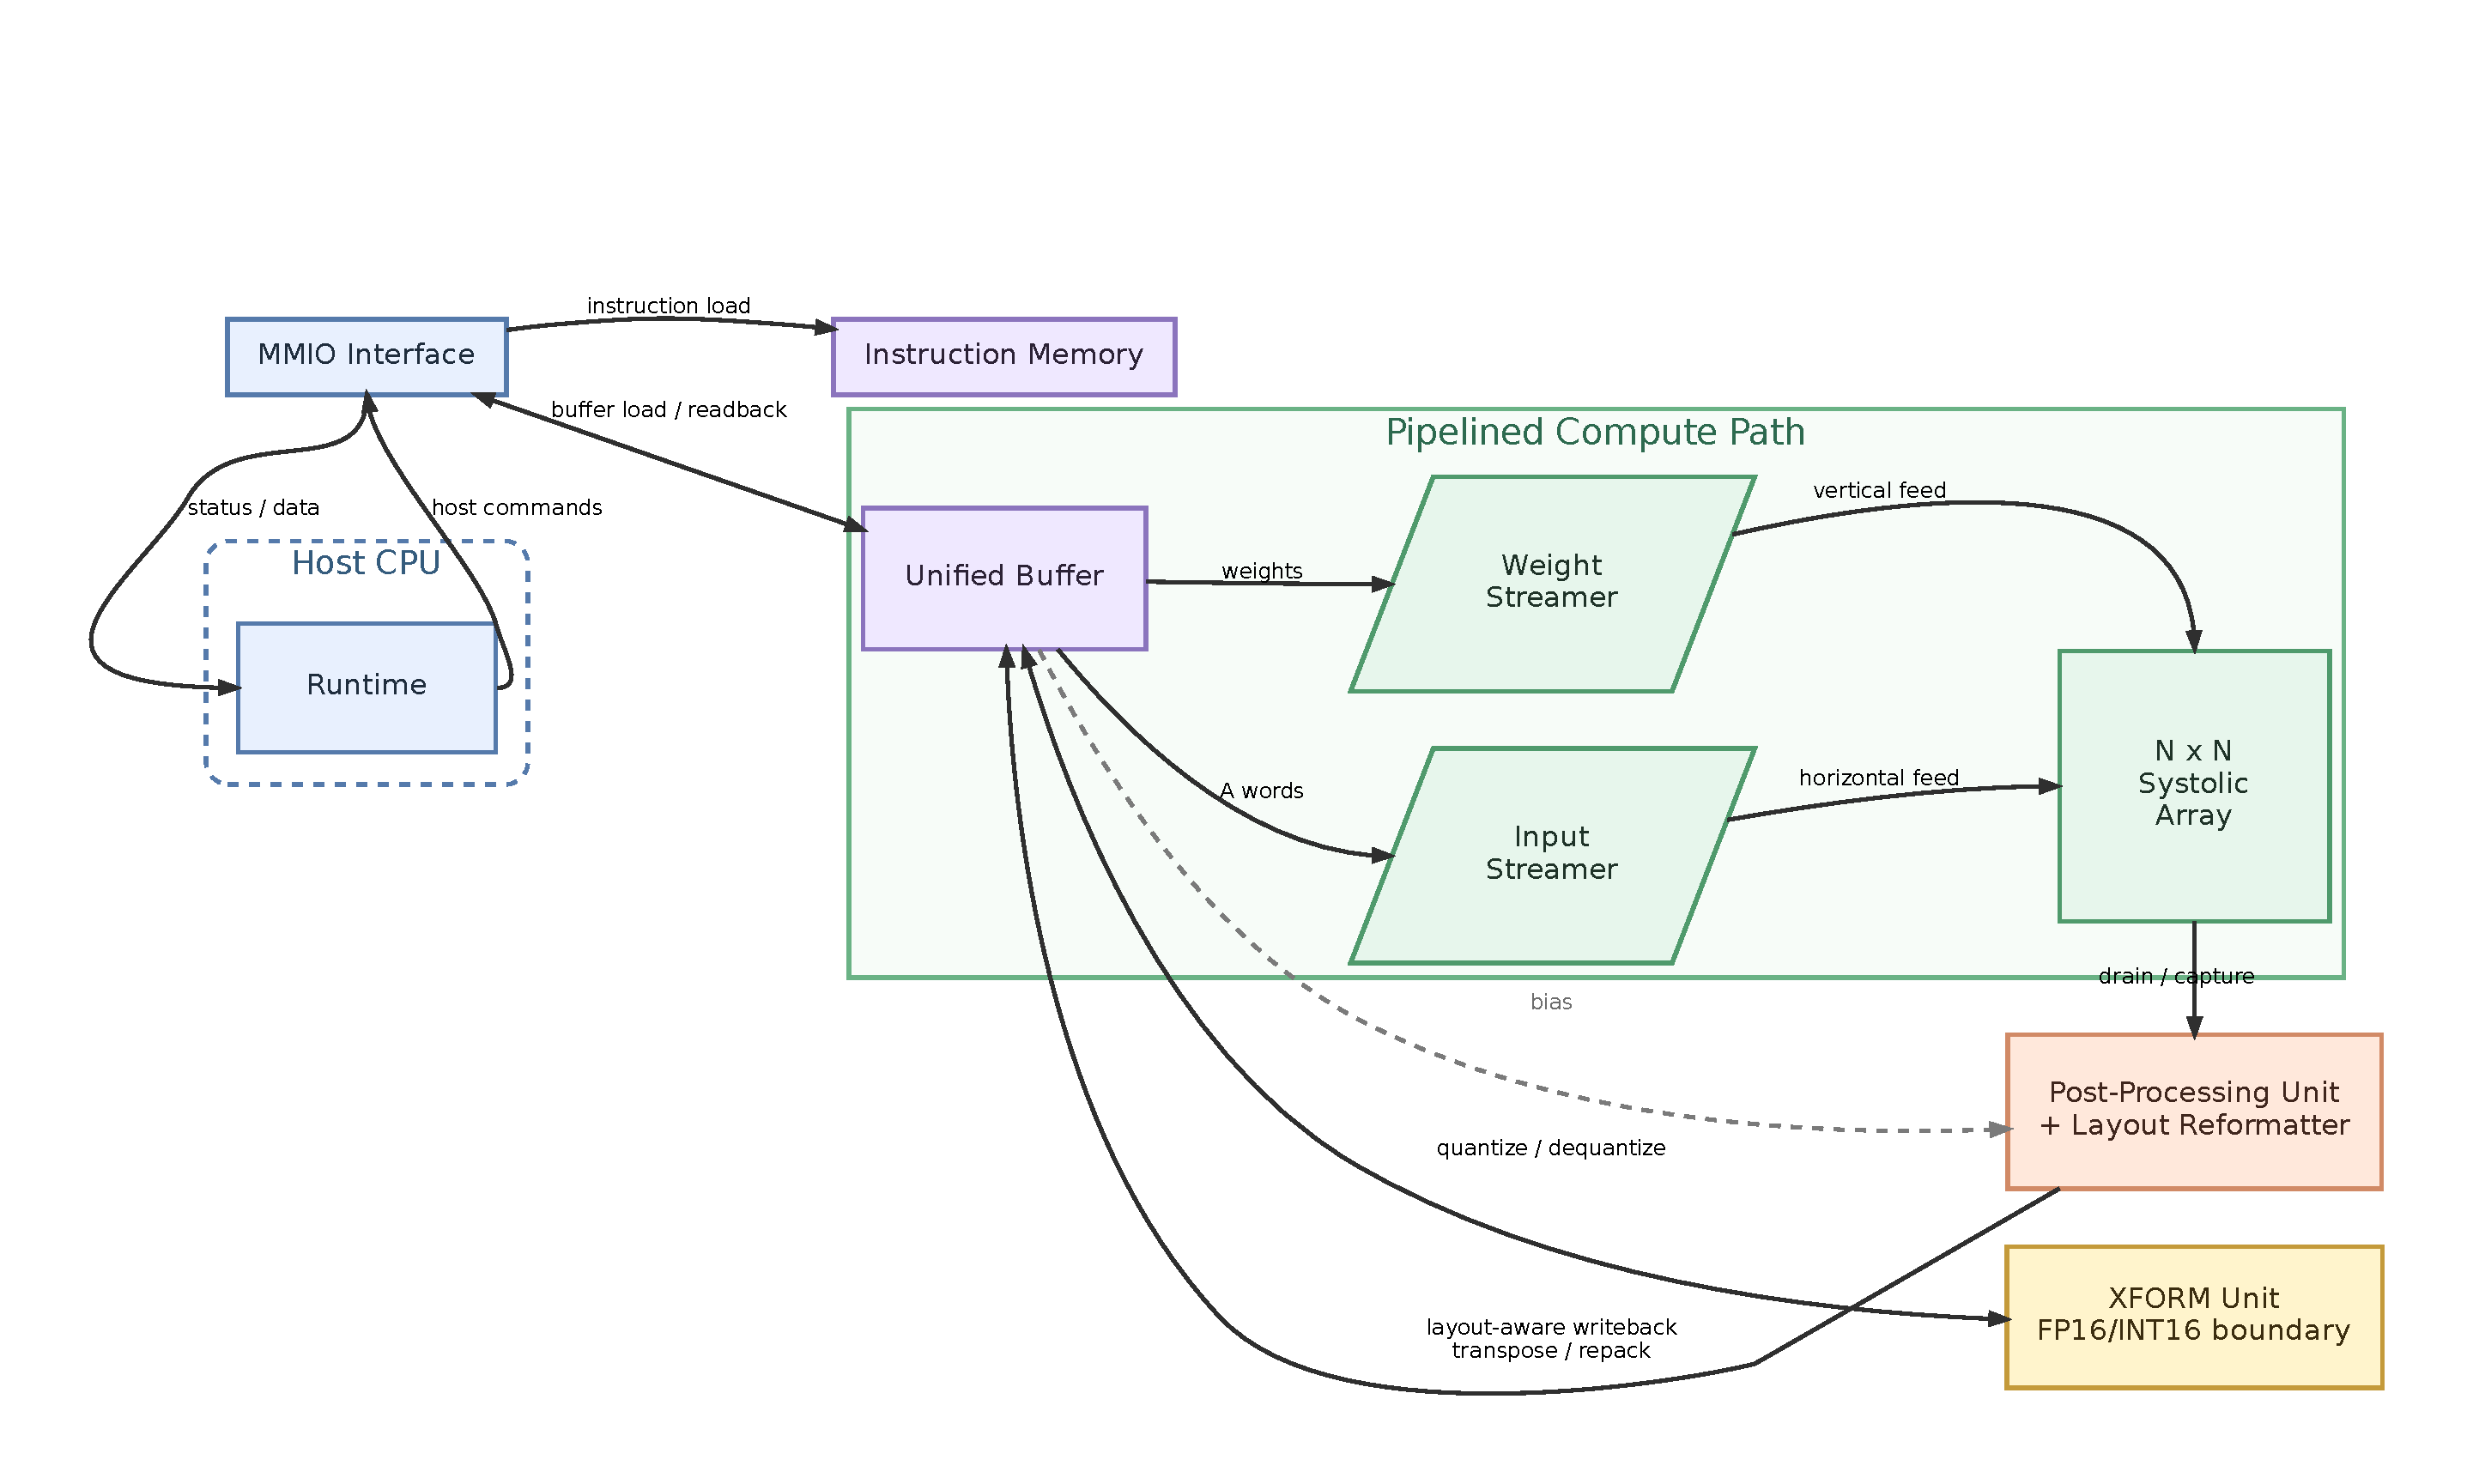
\includegraphics[width=\textwidth]{diagrams/hardware_architecture_graphviz.pdf}
    \caption{Top-level TinyNPU hardware architecture.}
    \label{fig:hardware-architecture}
\end{figure}

Figure~\ref{fig:hardware-architecture} shows the top-level organization used throughout this report. The host-side runtime communicates with the accelerator through the MMIO interface, which is responsible for instruction loading and buffer access. Inside the accelerator, the unified buffer, input streamer, weight streamer, and systolic array form the main pipelined compute path. The post-processing unit is shown separately because it becomes active during the later drain and writeback phase rather than during the main feed phase of the array. This distinction is important for explaining both data movement and measured execution cost.

The processing element itself is also structurally important to the project. Each PE supports packed low-precision arithmetic rather than only a single scalar multiply. In the current implementation, a PE can perform four INT4 products, two INT8 products, or one INT16 product in a step, and accumulates the resulting partial sum in stationary form. The array therefore gains speed not only from spatial parallelism across rows and columns, but also from packed arithmetic within each PE. This is one of the main reasons the accelerator can look strong on dense quantized kernels even though the surrounding system overhead is still significant.

Packing follows the same hardware structure. Activation-side data is packed to match the horizontal feed direction, weight-side data is packed to match the vertical feed direction, output storage is packed to match the writeback layout, and bias vectors are packed in wide words that match the post-processing path. This role-specific packing is not a cosmetic implementation detail. It is part of the architecture contract, and it strongly influences the compiler and runtime because legal execution depends on matching physical layout to the actual dataflow through the array and post-processing logic.

On the software side, the key structural idea is segmented execution. Instead of forcing the entire model into a single monolithic accelerator program, the compiler identifies supported regions and emits them as accelerator segments, while unsupported or intentionally host-resident work remains as host operations. This representation is simpler than a full whole-graph hardware-only compiler, but it makes the cost of boundaries, packing, and readback visible. The runtime then executes the plan step by step, coordinating accelerator launches and host computation as needed.

\begin{figure}[H]
    \centering
    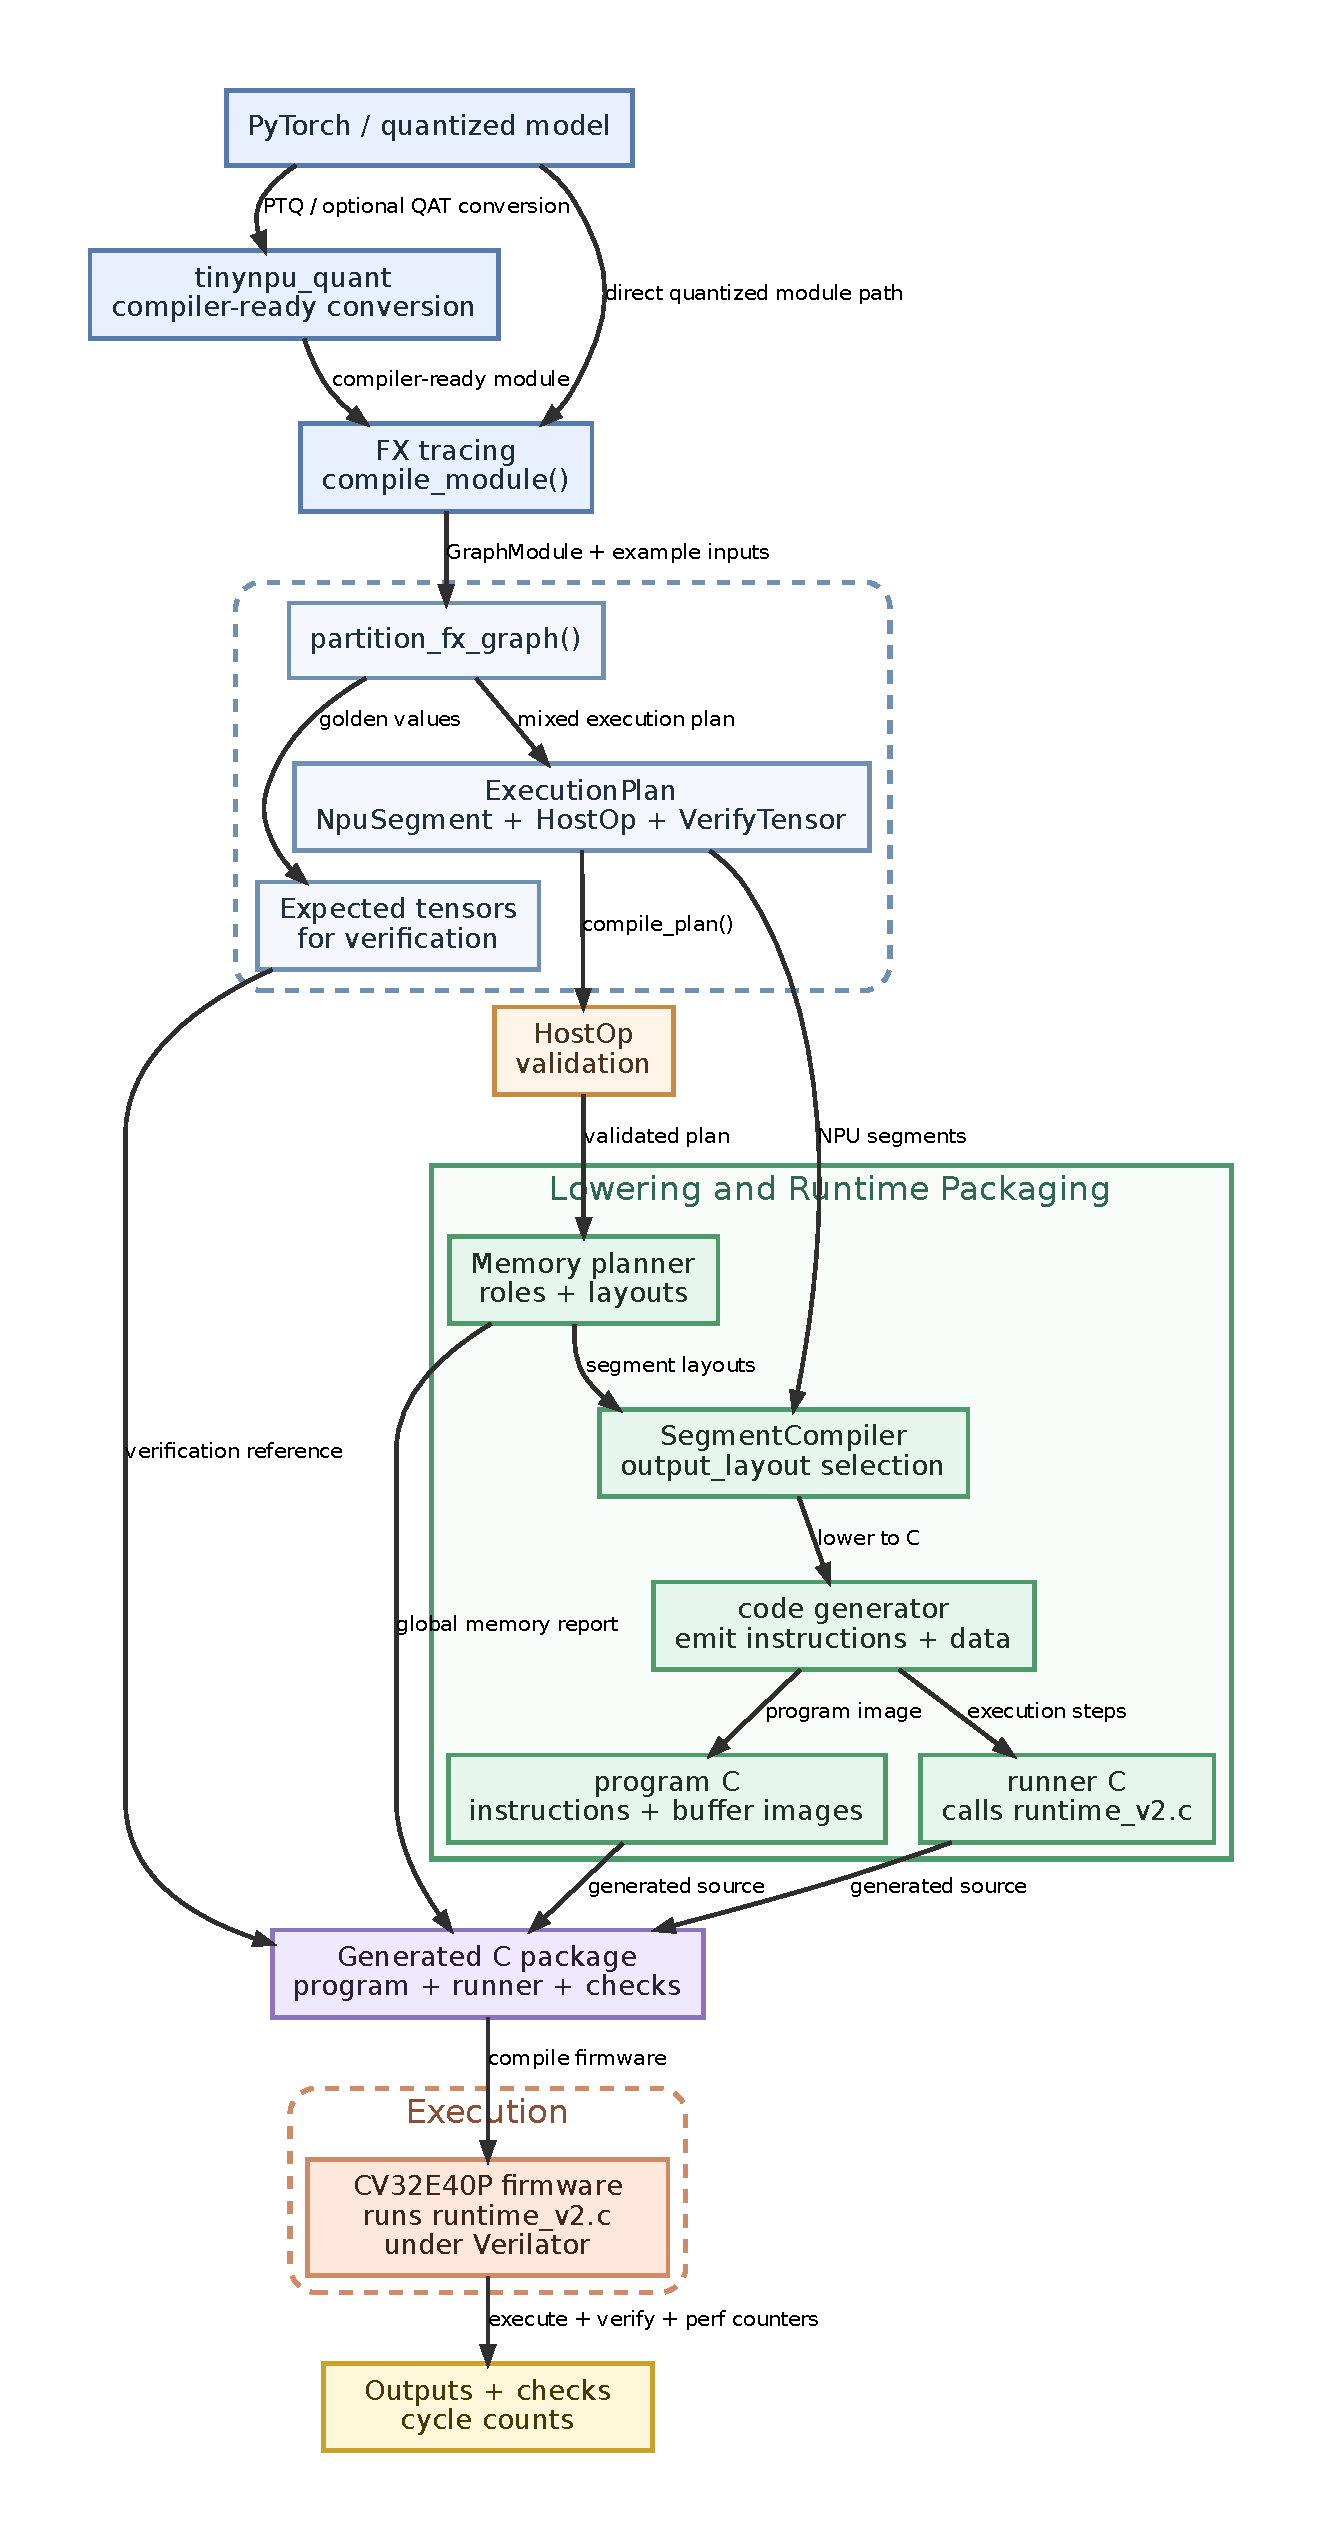
\includegraphics[width=0.92\textwidth,height=0.72\textheight,keepaspectratio]{diagrams/compiler_stack_graphviz.pdf}
    \caption{Compiler and runtime flow used by the TinyNPU JIT path.}
    \label{fig:compiler-stack}
\end{figure}

Figure~\ref{fig:compiler-stack} summarizes the software flow implemented in the repository. A model enters either directly as a supported quantized PyTorch module or through a compiler-ready conversion path built around \texttt{tinynpu\_quant}. The JIT frontend traces the model with FX, partitions it into a mixed execution plan, validates host operations, and lowers each accelerator segment through the memory planner and \texttt{SegmentCompiler}. The resulting \texttt{CompiledArtifact} contains the execution plan, per-segment IM/UB binaries, expected tensors for verification, and memory-layout information required by the runtime. The current emitter/runtime boundary is intentionally static-data-heavy: generated C files carry program tables and constants, while shared runtime code executes those tables through a fixed interpreter-style loop.

Another important structural choice is that benchmarking is built into the execution path. The runtime can collect hard RTL cycle counts for accelerator execution windows and keep separate accounting for software-side overhead such as buffer loading and packing. This allows the project to reason about compute efficiency without confusing it with prototype integration overhead.

\begin{figure}[H]
    \centering
    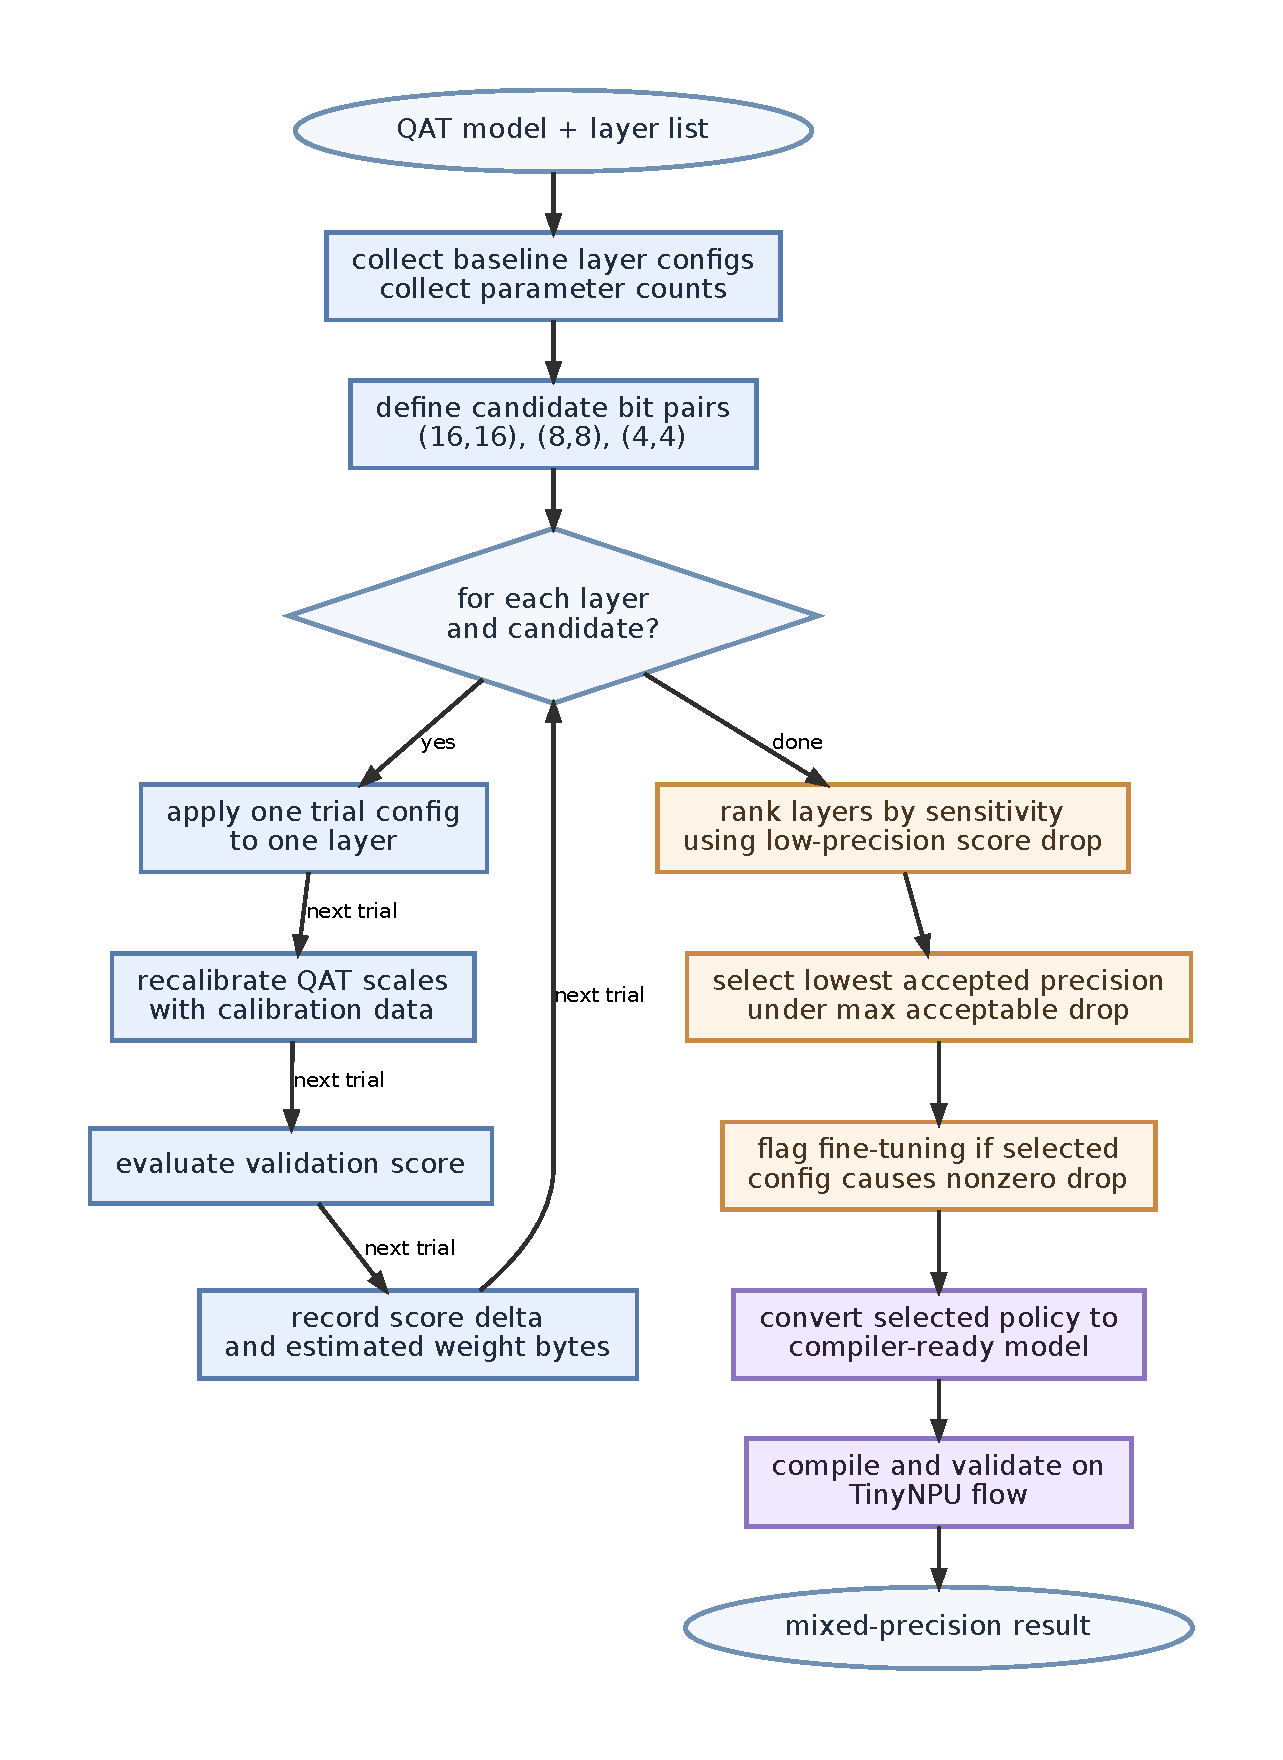
\includegraphics[width=0.88\textwidth,height=0.62\textheight,keepaspectratio]{diagrams/bit_selection_flow_graphviz.pdf}
    \caption{Heuristic mixed-precision selection flow used to obtain compiler-ready model variants.}
    \label{fig:bit-selection}
\end{figure}

Figure~\ref{fig:bit-selection} shows the mixed-precision selection helper currently used in the project. It is important to state its scope precisely. The project is not attempting to solve the general bit-allocation problem or to claim an optimal mixed-precision policy. Instead, it implements a simple one-layer-at-a-time sensitivity workflow that is sufficient to generate candidate mixed-precision configurations, recalibrate them, and feed the selected result into the compiler-ready conversion path. This keeps the project focused on obtaining usable results in the TinyNPU flow rather than overclaiming a global mixed-precision optimization method.
\subsection{Dynamic Model}
Dynamically, the system operates as a mixed host-accelerator execution pipeline. A prepared model is first converted into an execution plan. At runtime, the host loads instruction and buffer state, launches an accelerator segment, waits for completion, and then either proceeds to the next accelerator segment or executes a host operation. This continues until the final outputs are produced. The important point is that unsupported operations are not hidden. They are explicit runtime steps, which means their cost and semantic effect can both be observed and measured.

The same dynamic model also supports verification and repeated inference. Verification steps compare runtime tensors with compiler-owned expected tensors when the selected verification mode enables them. Repeated-run sessions allow the simulator backend to preserve reusable state such as static buffer contents and preloaded instruction images. This does not eliminate all setup cost, but it makes the runtime model more realistic for repeated inference and allows overhead reductions to be measured directly.

\begin{figure}[H]
    \centering
    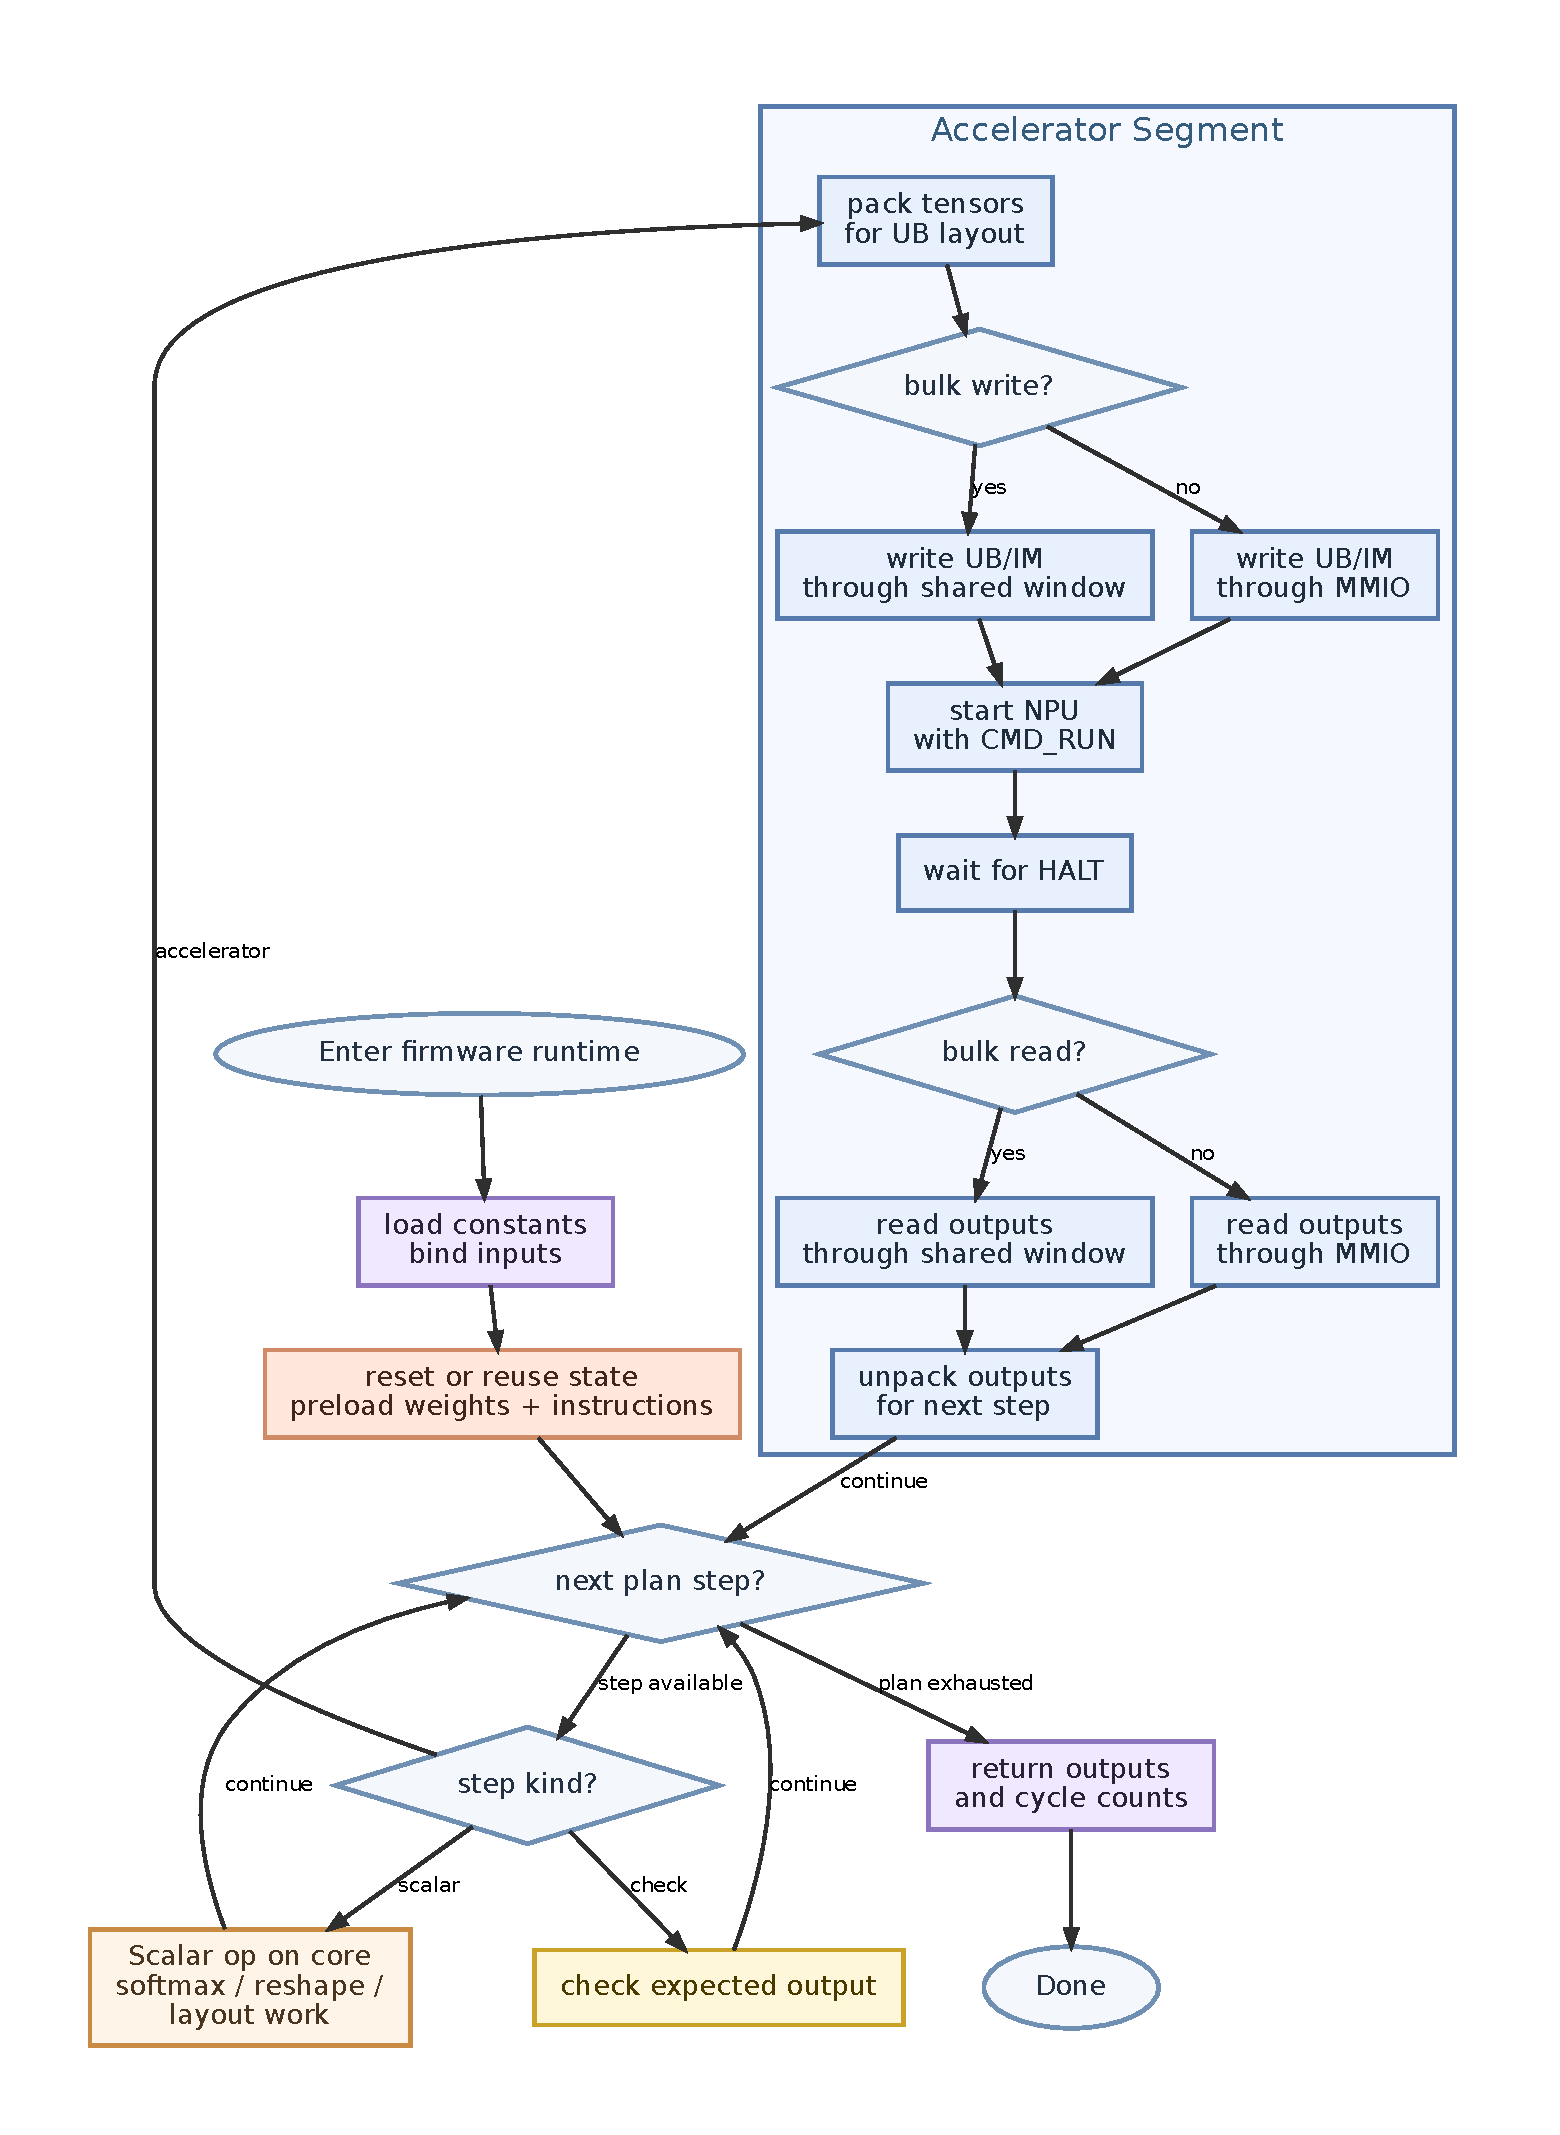
\includegraphics[width=0.9\textwidth,height=0.58\textheight,keepaspectratio]{diagrams/runtime_state_graphviz.pdf}
    \caption{Host-side runtime flow for executing a compiled TinyNPU artifact.}
    \label{fig:runtime-state}
\end{figure}

Figure~\ref{fig:runtime-state} shows the same runtime loop from the host-side orchestration perspective. For accelerator segments, the runtime first packs logical tensors into the physical layouts expected by the datapath, stages vectors into the unified buffer (shared-SRAM direct path by default, MMIO path as fallback), launches execution, waits for completion, and then reads and unpacks the resulting vectors back into logical tensors. Host-side operations such as requantization, dequantization, softmax, mean, and shape movement appear explicitly in the same loop rather than being hidden behind the accelerator interface. This view is more useful for discussing runtime overhead, because it makes the cost of packing, transfers, polling, and readback visible.

\subsubsection{Execution Phases}
From the hardware perspective, not every block is active at the same time. The unified buffer, streamer logic, and systolic array form the core pipelined compute path during active matrix-style computation. The post-processing unit participates during the later drain and writeback phase rather than during the main feed phase. This distinction matters for both architectural explanation and performance analysis, because the full accelerator latency is not just the array datapath alone.

From the runtime perspective, these phases are visible as distinct host-side responsibilities. Before the feed phase can begin, the runtime must pack logical tensors into accelerator-facing layouts and write the necessary vectors into the unified buffer. The runtime then issues the launch command and waits while the array consumes the streamed data. After the feed phase, outputs are drained through the post-processing unit, written back in packed form, and finally read and unpacked by the host runtime. This separation is important because it explains why accelerator compute cycles and runtime overhead must be measured separately.

\begin{figure}[H]
    \centering
    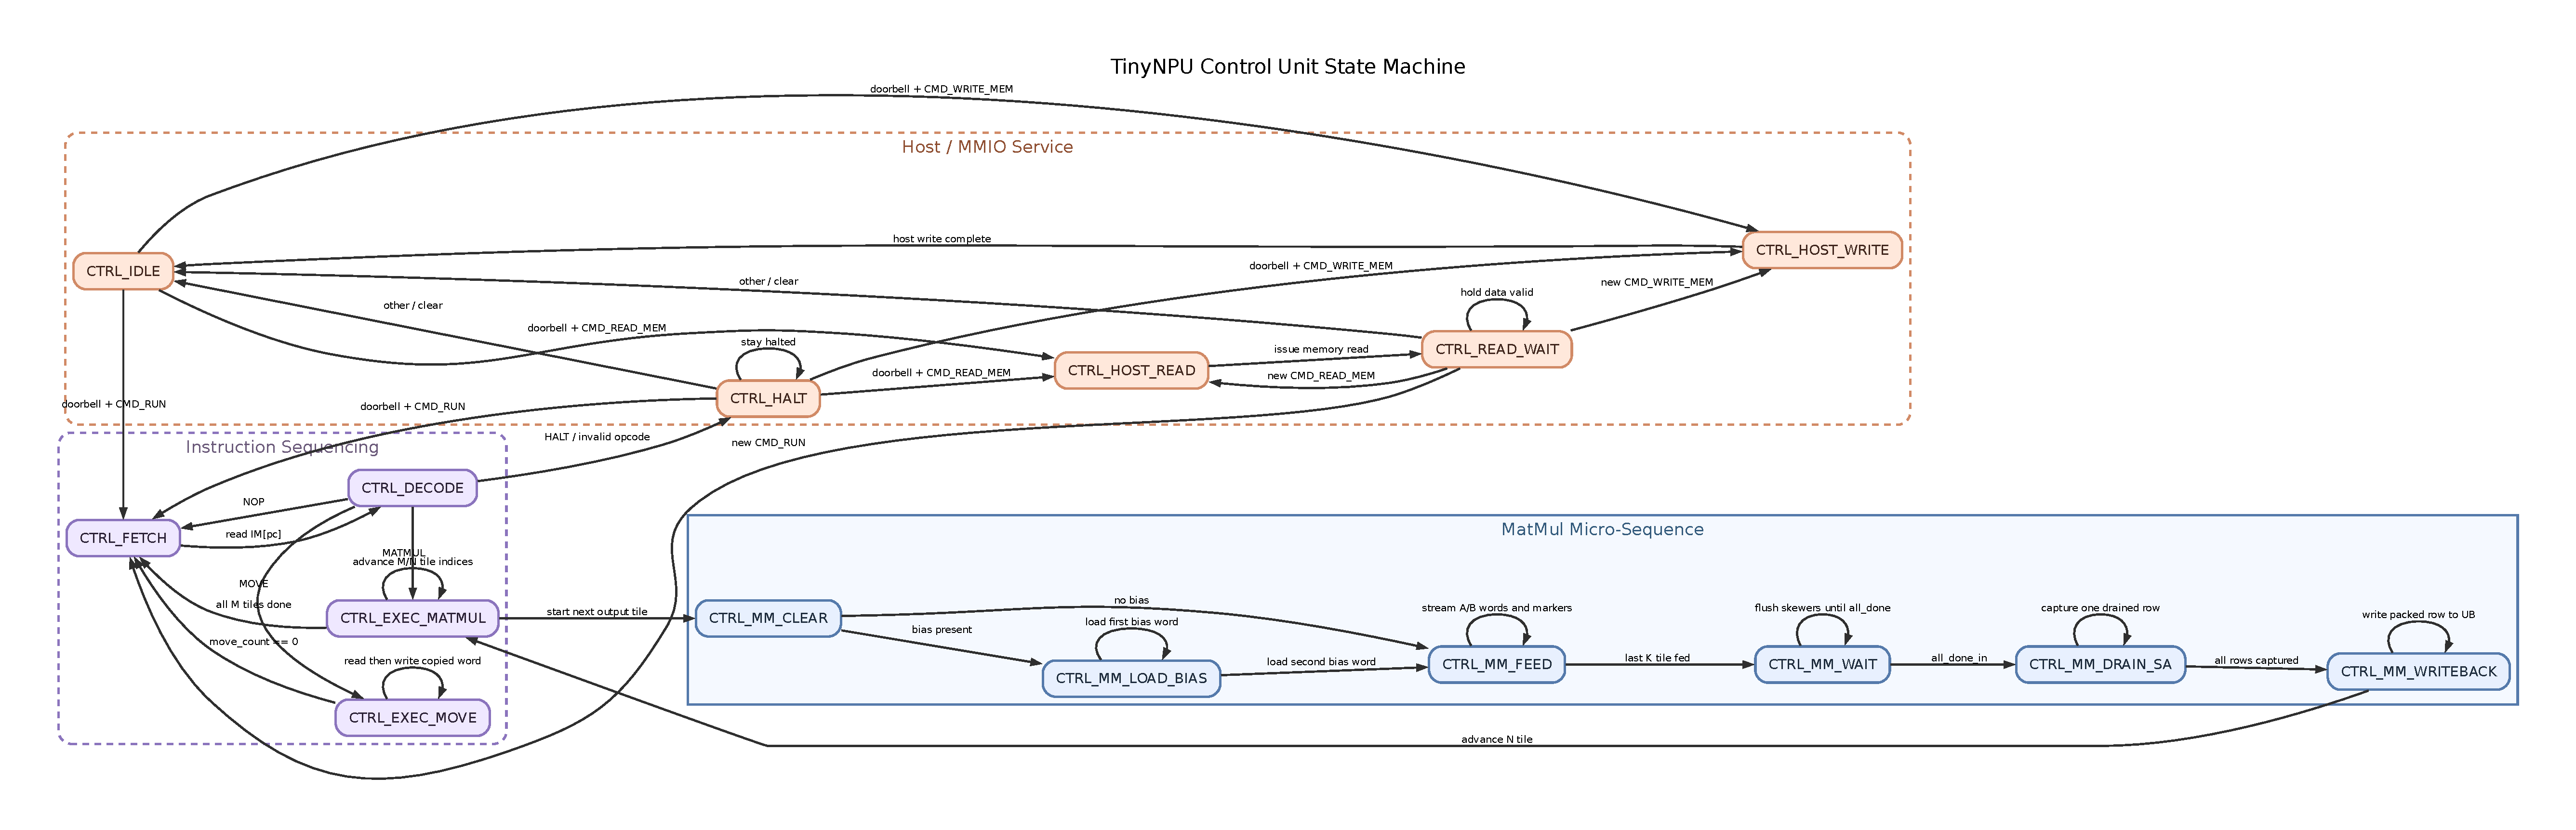
\includegraphics[width=\textwidth,height=0.46\textheight,keepaspectratio]{diagrams/control_states_graphviz.pdf}
    \caption{Control-unit states tracked by the internal performance counters, grouped by host service, instruction sequencing, and the matrix-multiplication micro-sequence.}
    \label{fig:control-states}
\end{figure}

Figure~\ref{fig:control-states} provides the hardware-side view of those phases. The host-visible states cover MMIO-driven writes, reads, and quiescent behavior. The instruction-sequencing states handle fetch and decode. Once a matrix multiplication begins, the controller moves through a more detailed micro-sequence including setup, optional bias load, feed, wait, drain, and writeback.

This state machine is not only descriptive; it is also observable. When performance monitoring is enabled, the control unit exposes a total cycle counter together with per-state cycle and entry counters. In other words, the project can record not just how long an accelerator segment took overall, but how that time was distributed across states such as \texttt{CTRL\_FETCH}, \texttt{CTRL\_DECODE}, \texttt{CTRL\_MM\_FEED}, \texttt{CTRL\_MM\_WAIT}, and \texttt{CTRL\_MM\_WRITEBACK}. This is useful because it makes the ``compute'' window interpretable rather than opaque: the measured accelerator run time still contains control and synchronization work in addition to the active datapath feed phase.

\begin{figure}[H]
    \centering
    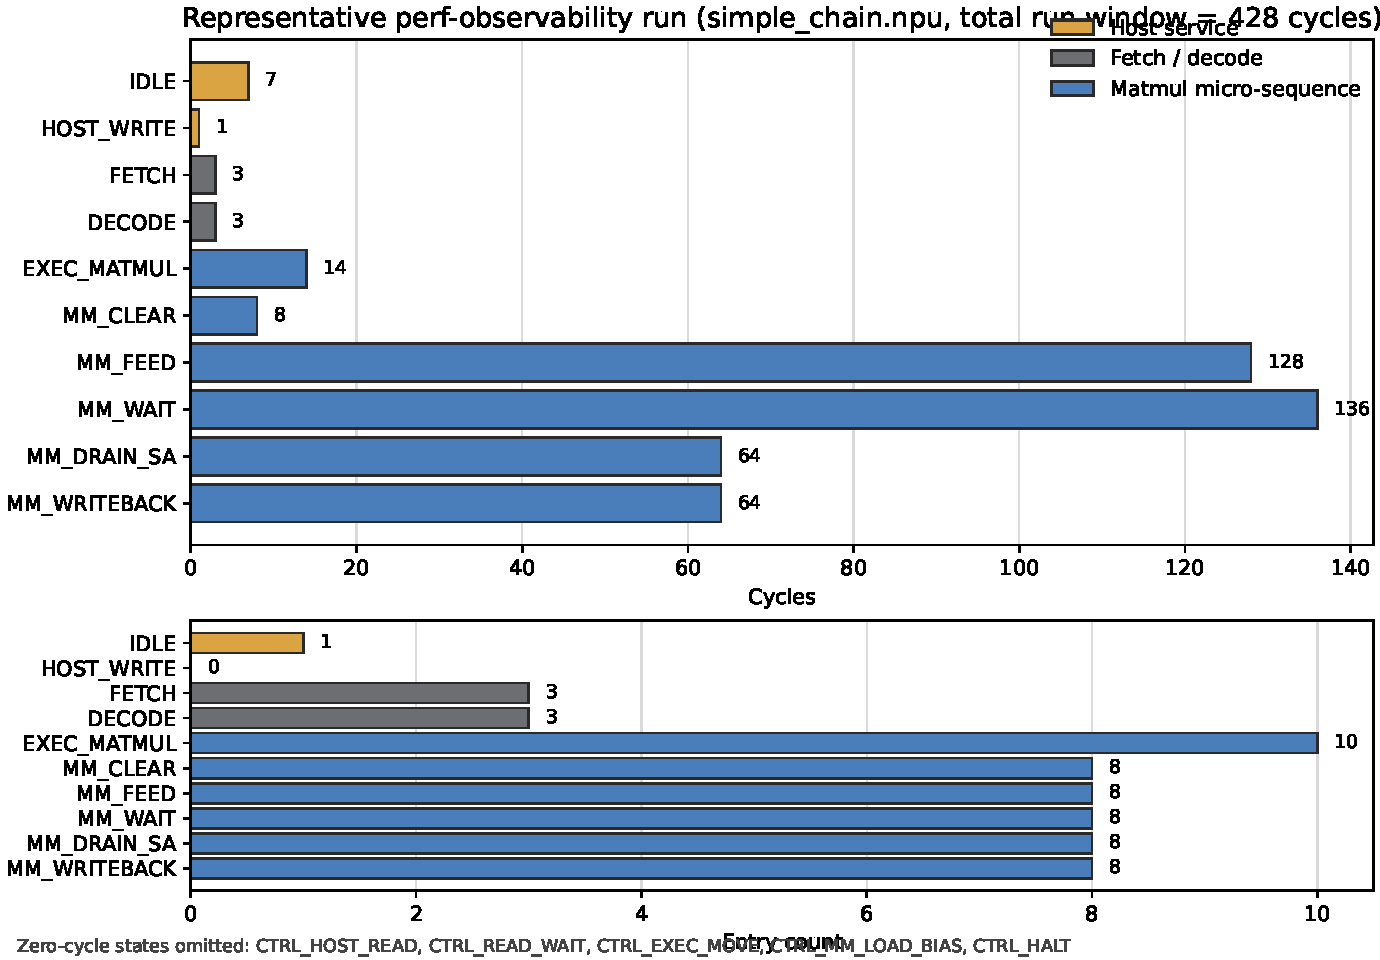
\includegraphics[width=0.96\textwidth,height=0.60\textheight,keepaspectratio]{diagrams/control_state_breakdown.pdf}
    \caption{Measured per-state cycle and entry breakdown for a representative perf-observability run on \texttt{simple\_chain.npu}. Zero-cycle states are omitted for readability.}
    \label{fig:control-state-breakdown}
\end{figure}

Figure~\ref{fig:control-state-breakdown} turns that observability mechanism into an actual measurement. In this representative run, the dominant states are \texttt{CTRL\_MM\_FEED} and \texttt{CTRL\_MM\_WAIT}, which together account for 264 of the 428 measured cycles. The drain and writeback phases contribute another 128 cycles. By contrast, fetch and decode are only 6 cycles in total, and host-visible service states are negligible inside the measured run window. This is exactly the kind of visibility needed to reason about whether performance is limited by active streaming, array fill and drain behavior, or surrounding control overhead.

\subsubsection{Current Scope Boundaries}
The current system is deliberately narrower than a general-purpose deployment stack. The mixed-precision helper is meant to produce usable compiler-ready configurations, not to solve the global bit-allocation problem. The compiler handles a bounded set of operators and makes unsupported behavior explicit through host operations rather than pretending to provide transparent full-model lowering. Workload coverage is also still narrow: the current report is grounded in one end-to-end model case and one controlled kernel benchmark. These limitations are acceptable for the present project scope because the main objective is to build and understand a working accelerator system, not to claim a finished production compiler.

\newpage
\section{Experimental Setup and Design} 
The project was evaluated primarily in simulation, using both host-side execution and RTL-backed cocotb tests. This was necessary because the main goal of the project is not only to confirm functionality, but also to understand how compiler decisions, packing format, and runtime policy affect accelerator behavior before any physical implementation is assumed. Host emulation and RTL simulation share the same execution-plan concept, which made it possible to compare compiler behavior against a golden software model while still collecting hardware-facing evidence.

The experimentation setup contains three layers. First, unit and regression tests validate compiler transformations, execution-plan behavior, memory-planning behavior, and host-op semantics. Second, RTL simulation validates full hardware/software interaction and allows performance counters to be read during accelerator execution. Third, a reproducible Yosys-based synthesis flow provides rough logic and resource estimates for the current top-level design both with and without treating the major memories as abstract macros.

The RTL performance-monitoring path is particularly important for interpreting the accelerator measurements. With performance monitoring enabled, the control unit reports not only a total run-window cycle count, but also per-state cycle and entry counts for its internal control states. This makes it possible to distinguish broad classes of activity such as host service, fetch/decode, feed, wait, drain, and writeback when analyzing where the accelerator is actually spending time during a segment.

The current empirical evidence is intentionally limited and should be described honestly in the report. There is one full end-to-end model case study: a trained MNIST flow that passes through model preparation, compiler-ready conversion, segmented compilation, and RTL-backed validation. There is also one controlled performance case study: a multi-tile matrix multiplication workload large enough to force tiling on the current array configuration. This benchmark is not intended to represent full-model latency by itself; it is a kernel-level workload chosen to isolate the accelerator’s core behavior and the effect of integration overhead.

The performance methodology separates different cost categories on purpose. Accelerator compute cycles are taken from RTL performance counters during the run window of a segment. Software-side overhead such as loading buffer images, issuing control transactions, packing and unpacking data, and executing host-only operations is accounted for separately. Several CPU reference models are also applied on the software side, but these are analytic comparison models rather than measurements from a physical reference processor. The purpose of those models is to bound and interpret the accelerator’s behavior, not to claim a definitive CPU-versus-NPU benchmark.

For the refreshed runtime-coverage runs in this report, all firmware binaries were built with \texttt{-march=rv32imfc -mabi=ilp32 -O3} and \texttt{-DTNPU\_RUNTIME\_V2\_DUMP\_FINAL\_OUTPUTS=0}. Runtime validation used \texttt{autoverify} against compiler-owned expected tensors when explicit verify ops were not emitted. The simulation command was fixed at \texttt{VERILATOR\_MAX\_TICKS=3000000000} with \texttt{+maxcycles=250000} to keep runs directly comparable.

\newpage
\section{Comparative Evaluation and Discussion}
The current evaluation supports several concrete conclusions, but it should be read with the correct scope. The evidence is sufficient to show that the stack works end to end and that the accelerator core is meaningful. It is not yet broad enough to support sweeping claims about general workload coverage.

First, the end-to-end software and hardware path is real. A trained MNIST model has been prepared for the compiler, compiled through the segmented JIT flow, and validated against RTL. This is important because the central claim of the project is not simply that individual kernels run, but that a model can move from PyTorch-side preparation into a real TinyNPU execution artifact and still preserve host/RTL correctness.

Second, the performance tooling reveals a clear separation between core compute strength and integration cost. On the current multi-tile matrix multiplication benchmark, the RTL run window for the accelerator is only 369 cycles. Depending on the chosen CPU reference model, this translates to a large pure compute speedup range, but the integration-adjusted speedup is much lower because runtime and protocol overhead still matter. This is exactly the kind of conclusion the benchmark path was designed to support: the datapath itself may be strong, while the surrounding software and interface contract still leave room for improvement.

\begin{table}[H]
    \centering
    \caption{Controlled multi-tile matrix multiplication benchmark results for the $13 \times 17$ by $17 \times 19$ workload.}
    \label{tab:matmul-benchmark}
    \begin{tabularx}{\textwidth}{|l|Y|Y|Y|}
        \hline
        \textbf{Reference model} & \textbf{CPU replaced cycles} & \textbf{Pure acceleration speedup} & \textbf{Integration-adjusted speedup} \\
        \hline
        Unpipelined scalar & 51870 & 140.57$\times$ & 8.39$\times$ \\
        \hline
        Ideal issue-1 & 30628 & 83.00$\times$ & 5.20$\times$ \\
        \hline
        Five-stage in-order & 43472 & 117.81$\times$ & 7.09$\times$ \\
        \hline
    \end{tabularx}
\end{table}

For the same workload, the measured accelerator run window was 369 cycles. Table~\ref{tab:matmul-benchmark} makes the key point visible: the compute core itself is strong, but integration-adjusted speedup is much lower than pure compute speedup because runtime and interface costs are still substantial.

Third, repeated-run runtime work is already justified by measured behavior. On a small repeated-run benchmark, static persistence reduced the modeled NPU-side overhead from 3036 to 1744 units, which corresponds to roughly a 42.6\% reduction. On trained MNIST, where the workload is more activation-heavy, the same idea still reduced repeated-run unified-buffer traffic from 17608 words to 14920 words, which is about a 15.3\% reduction. These numbers do not claim that the whole problem is solved; they show that repeated-run state reuse is a real and measurable optimization direction.

\begin{table}[H]
    \centering
    \small
    \caption{Observed effect of repeated-run persistence on two workloads.}
    \label{tab:persistence-results}
    \begin{tabularx}{\textwidth}{|l|l|Y|Y|Y|}
        \hline
        \textbf{Workload} & \textbf{Metric} & \makecell{\textbf{Baseline}} & \makecell{\textbf{Persistence}\\\textbf{path}} & \makecell{\textbf{Observed}\\\textbf{effect}} \\
        \hline
        Small repeated-run artifact & NPU overhead cycles & 3036 & 1744 & 42.6\% lower overhead \\
        \hline
        Trained MNIST & UB words per run & 17608 & 14920 & 15.3\% lower steady-state traffic \\
        \hline
    \end{tabularx}
\end{table}

Fourth, the current runtime correctness baseline was re-checked after the packed conv-stream RTL fix. Table~\ref{tab:runtime-coverage-refresh-interim} reports the refreshed matrix under one fixed build/run method. The practical result is clear: direct INT16 and direct packed INT8 are stable, and direct packed INT4 is also stable when fixtures obey signed INT4 range limits.

\begin{table}[H]
    \centering
    \footnotesize
    \caption{Runtime coverage refresh after packed conv-stream RTL update.}
    \label{tab:runtime-coverage-refresh-interim}
    \begin{tabularx}{\textwidth}{|>{\raggedright\arraybackslash}X|l|r|r|r|r|r|l|}
        \hline
        \textbf{Program} & \textbf{Path} & \textbf{Host Im2Col} & \textbf{Stage} & \textbf{Run} & \textbf{Readback} & \textbf{Seg.NPU} & \textbf{Verify} \\
        \hline
        \texttt{cv32e40p\_int16\_convstream\_same\_shape\_v2} & conv-stream & 0 & 3810 & 530 & 3387 & 13707 & OK \\
        \hline
        \texttt{cv32e40p\_int8\_packed\_convstream\_default\_v2} & direct packed conv-stream & 0 & 7309 & 98 & 2931 & 16267 & OK \\
        \hline
        \texttt{cv32e40p\_int4\_convstream\_same\_shape\_v2} & host \texttt{im2col} + NPU & 52988 & 40004 & 290 & 9453 & 55821 & OK \\
        \hline
        \texttt{cv32e40p\_int4\_packed\_convstream\_default\_v2\_inrange} & direct packed conv-stream & 0 & 9176 & 82 & 3199 & 18386 & OK \\
        \hline
        \texttt{cv32e40p\_int4\_packed\_convstream\_default\_v2} & direct packed conv-stream & 0 & 9176 & 82 & 3195 & 18382 & FAIL (\texttt{@0}) \\
        \hline
    \end{tabularx}
\end{table}

The one remaining INT4 failure in the table is a fixture-validity issue (\texttt{xmat} in \([-14,14]\), outside signed INT4 \([-8,7]\)) rather than a datapath mismatch.

Fifth, the synthesis-oriented characterization confirms that the design is no longer trivial in hardware terms. Under the reproducible Yosys flow, the top-level design synthesized to an estimated 25117 logic cells when the major memories were abstracted and 33644 logic cells when the current memory implementation was kept, with 227 DSP48 blocks in both cases. These numbers are only rough synthesis proxies, not final silicon area, but they are enough to show that TinyNPU is a substantial compute block whose area and timing behavior now deserve serious attention.

The most important interpretation of these results is that the project’s center of gravity has shifted. The compiler and runtime exist well enough to run real workloads. The pressing questions are now about workload fit, cycle reduction, memory sizing, and hardware cost, not about whether a compiler path can exist at all.

\newpage
\section{Conclusion and Future Work}
TinyNPU has reached the point where it should be treated as a real accelerator platform rather than as a collection of disconnected experiments. The project now contains a usable hardware architecture, a PyTorch-oriented model preparation flow, a segmented compiler/runtime, explicit host-boundary handling, repeated-inference support, verification infrastructure, and benchmark tooling capable of separating compute from overhead. That is a substantial transition from the early stage of simply proving that isolated RTL blocks or simple kernels behaved correctly.

At the same time, the project makes its own limitations visible in a useful way. The current system still pays a noticeable cost for segmentation, state movement, packing, and host-visible boundaries. The mixed-precision path is practical for preparing compiler-ready models, but it is not intended to solve the global bit-allocation problem. Workload coverage is still narrow, and the current performance story is based on one end-to-end model and one controlled kernel benchmark rather than on a broad suite of models.

Those limitations point directly to the next phase of work. The highest-value future work is no longer ``make the compiler exist.'' It is to bring more models onto the stack, reduce avoidable runtime and interface overhead, increase the size of useful accelerator regions, and use real workloads to justify changes in unified-buffer and instruction-memory sizing. On the hardware side, synthesis and timing characterization should be extended beyond rough proxy numbers. On the software side, additional compiler work should be driven by measured workload needs rather than by abstraction for its own sake. That is the most credible path forward for TinyNPU as a research system.

\newpage
\bibliographystyle{plain}
\bibliography{references} 

\end{document}
